%%%%%%%%%%%%%%%%%%%%%%%%%%%%%%%%%%%%%%%%%%%%%%%%%%
%% Bachelor's & Master's Thesis Template        %%
%% Copyleft by Dawid Weiss & Marta Szachniuk    %%
%% Faculty of Computing and Telecommunication   %%
%% Poznan University of Technology, 2020        %%
%%%%%%%%%%%%%%%%%%%%%%%%%%%%%%%%%%%%%%%%%%%%%%%%%%

\documentclass[english,bachelor,a4paper,oneside]{ppfcmthesis}


\usepackage[utf8]{inputenc}
\usepackage[OT4]{fontenc}
\usepackage{graphicx}
\usepackage{hyperref}
\usepackage{float}
\usepackage{tikz}
\usepackage{amsmath}
\usetikzlibrary{shapes.geometric, arrows}

% Define styles
\tikzstyle{startstop} = [rectangle, rounded corners, minimum width=3cm, minimum height=1cm, align=center, draw=black, fill=blue!30]
\tikzstyle{process} = [rectangle, minimum width=3cm, minimum height=1cm, align=center, draw=black, fill=blue!30]
\tikzstyle{arrow} = [thick,->,>=stealth]

% 
\usepackage{xcolor}
\newcommand\myworries[1]{\textcolor{red}{#1}}
%

%--------------------------------------
% Strona tytułowa
%--------------------------------------

% Autorzy pracy, jeśli jest ich więcej niż jeden
% wstaw między nimi separator \and
\author{%
   Jakub Grabowski \album{151825} \and 
   Filip Kozłowski \album{151823} \and 
   Krzysztof Matyla \album{151778} \and 
   Igor Warszawski \album{151585}}
\authortitle{}                                % Do not change.

\title{Biometric identification of a smartphone user using graph neural networks}

% Your supervisor comes here.
\ppsupervisor{~dr hab.~inż.~Szymon Szczęsny, ~prof. PP} 

% Year of final submission (not graduation!)
\ppyear{2025}                                 


\begin{document}

% Front matter starts here
\frontmatter\pagestyle{empty}%
\maketitle\cleardoublepage%

%--------------------------------------
% Miejsce na kartę pracy dyplomowej
%--------------------------------------

\thispagestyle{empty}\vspace*{\fill}%
\begin{center}Tutaj będzie karta pracy dyplomowej;\\oryginał wstawiamy do wersji dla archiwum PP, w pozostałych kopiach wstawiamy ksero.\end{center}%
\vfill\cleardoublepage%

%--------------------------------------
% Spis treści
%--------------------------------------

\pagenumbering{Roman}\pagestyle{ppfcmthesis}%
\tableofcontents* 
\cleardoublepage % Zaczynamy od nieparzystej strony

%--------------------------------------
% Rozdziały
%--------------------------------------

%Najwygodniej jeśli każdy rozdział znajduje się w oddzielnym pliku
\mainmatter%

\chapter{Introduction}

Biometric data is a widely used -- especially on mobile devices -- for user authentication. It is also used for person recognition. As of 2020, the majority of smartphones had biometric sensors, such as fingerprint readers \cite{statista_biometric_phones_2025}. Many computers can also provide biometric authentication via face recognition, if connected to a webcam, e.g. via Windows Hello on Windows 10 or 11 \cite{microsoft_windows_hello_2025}. These are, however, not the only possible recognition or authentication methods that use biometric data.

The project aimed to develop a model, along with a corresponding mobile app, capable of recognizing users based on their biometric data, primarily derived from keystroke patterns. Participants in the study, conducted as a part of the project, provided their data by entering long stretches of text as testing data. Models were created for each user, with the standard model testing procedures and validations. A subgroup of the study participants was also asked to verify the model in real-life testing by writing short paragraphs in the application, which were sent to the server for user verification.

The scope of the work was to create a mobile application capable of gathering the keystroke data, which could then be used by the server to create Graph Neural Network (GNN) models tasked with recognizing the user as opposed to other possible users. Also in the scope was performing a study on a group of participants who provided the data for the project and participated in the application and model demonstration and testing.

The sources referenced in this thesis primarily fall into two categories: studies on keystroke data models and their effectiveness, and specialist literature concerning Graph Neural Networks.

The thesis has the following structure:
\begin{itemize}
    \item Chapter 2 consists of some theory concerning biometrics, especially in the context of user input data, with a small literature review about using biometrics for user recognition.
    \item Chapter 3 contains basic theoretics about Graph Convolutional Networks, which are used for user recognition in the model created for the project.
    \item Chapter 4 is an overview of the project, explaining its components and the relationships between them. It contains subchapters about project use cases, server architecture and mobile application architecture.
    \item Chapter 5 is concerned with the Neural Network model, its design and feature engineering.
    \item Chapter 6 contains results of the study conducted on the users, with subchapter dedicated to discussing the findings.
    \item Chapter 7 is a brief conclusion to the thesis.
\end{itemize}

The division of labor for this project was as follows:
\begin{itemize}
    \item Jakub Grabowski created the mobile application, set up and coordinated the project, and researched biometrics for the thesis paper. He wrote chapters 1, 2, 7 and parts of chapters 3 and 6.
    \item Filip Kozłowski created the server and integrated the GNN model with it. He also planned and implemented communication between the server and the application. He wrote parts of chapters 3, 4 and 6. 
    \item Krzysztof Matyla helped in creating the mobile application interface, provided testing for various parts of the project, and coordinated user testing. He wrote most of chapter 4.
    \item Igor Warszawski planned and implemented the GNN model used on the server. He also tested and validated the results, together with Filip Kozłowski. He wrote chapter 5 and parts of chapters 3 and 6.
\end{itemize}


\chapter{Biometrics in mobile devices - theory}

Fundamental to the goal of the project was the use of biometric data in user identification. Biometric data can be defined as measurements of some unique characteristics of an individual. These can largely be divided into two main categories: physiological data, which is the measurement of the inherent characteristics of an individual's body, such as a fingerprint, an iris scan or a face scan, and behavioral data, which measures the person's movements, behaviors, speech patterns etc. \cite{Abde2023}

Uniqueness of one's body is well known in biology. Features that may be used for person's identification are for example (FIX SOURCE: https://www.biometricsinstitute.org/what-is-biometrics/types-of-biometrics/):

\begin{enumerate}
    \item \textbf{DNA} -- found in cells of the living organisms, this acid carries genetic information.
    \item \textbf{Eye features} -- human iris, retina and scleral veins can be used in eye scans.
    \item \textbf{Face} -- full face scan is often used for user recognition, for example in mobile devices and laptops. (FIX SOURCE: https://developers.google.com/ml-kit/vision/face-detection, https://support.apple.com/en-us/102381)
    \item \textbf{Fingerprints and finger shape} -- fingerprints are widely used in forensics (FIX SOURCE: https://www.nist.gov/forensic-biometrics) and in digital scanners on mobile devices and laptops.
\end{enumerate}

Other, less popular ways of identifying a person are for example: ear shape, gait, hand shape, heartbeat, keystroke dynamics, signatures, vein scans and voice recognition.

One possible way to extract data from a person's behavior is via *keystroke dynamics*. This type of behavioral biometrics is acquired from a user by means of a keyboard or other typing device and records and extracts features from the way the keyboard is used. Most commonly used and almost universally applicable to any keyboard device is the measurement of timings between each character typed. If the user uses a physical keyboard, it is also convenient to derive the following features \cite{Shar2023}:

\begin{enumerate}
    \item \textbf{Hold Time} -- time between key press and release
    \item \textbf{Down-Down Time} -- time between first key press and second key press
    \item \textbf{Up-Up Time} -- time between first key release and second key release
    \item \textbf{Up-Down Time} -- time between first key release and second key press
    \item \textbf{Down-Up Time} -- time between first key press and second key release.
\end{enumerate}


With some keyboards it may be more difficult to gather all the possible features. Even basic feature, such as the hold time can prove difficult when using for example GBoard on mobile devices, which does not naturally send key press and key release information to the application. This information can thus only be gathered in approximation or by building another virtual keyboard application. This, however, has its drawbacks. The users are generally used to one type of keyboard (on mobile it may be for example GBoard or SwiftKey), so forcing them to use another type of keyboard may be detrimental.

While the model may be less accurate because of the lack of features, there can be some ways to mitigate it. Some other features can be added, which are largely specific to mobile devices, such as accelerometer data, or a larger sample can be used. A few of those options were considered by the researchers, and the results will be discussed in the next chapters (chapters 3.3 to 3.5).

The keystroke identification can also rely on other data gathered from the keyboard, such as the specifics of letters used, their average frequencies, most common connections between the letter or other statistics \cite{Wang2024}. These statistics can be modeled in many ways. If the average Up-Up Time between two keys is gathered from the data, a graph can be formed, having additional features as see fit by the designers. Such graphs were constructed for the Neural Network models constructed in this study, which will be discussed in the next chapter.

Some biometric recognition methods have been described as "too intrusive" and are being questioned from the ethical standpoint. Additionally, data sourcing for Machine Learning models used for many biometric methods should also be ethically sourced (FIX SOURCE: EU GUIDELINES). In this study, all data was sourced from willing participants and anonymized using unique ID numbers given to the participants by the researchers.

Same person may write somewhat differently on different keyboards and machines. This study has a small subsection on cross-smartphone compatibility of the model.

\chapter{Graph Convolutional Networks}

Graphs can defined as mathematical structures $G$ consisting of a set of vertices $V$, a set of edges $E$ and an incidence function $\phi$, along with many variations and generalizations to such structure, can be used for describing entities, which are related to each other in some way. An example of such model could be a computer network graph or citation network. Neurons can also be modelled in a similar way. Relation data can often be best described using such graphs. \cite{Lesk2024}

Some problems relating to such data can be solved using Convolutional Neural Networks -- this can also be the case for keystroke dynamics data, such as with Lu et al. \cite{Lu2020} or Sharma et al. \cite{Shar2023}. However, it can be reasoned that the Graph Neural Networks can also perform such tasks, with connections in graph data being used more directly in the model itself.

\section{Graph Neural Networks}
Graph Neural Networks (GNNs) are designed for graph inputs. The resulting outputs are also graphs (specifically, they are node embeddings representing a graph), allowing for transforming information in the graph's nodes, edges and global context, such as metadata about the graph, aggregated information, graph features etc. \cite{sanch2021}. GNN do not change the connectivity of the input in the output. 

Graphs in GNNs are represented with two main components: the adjacency matrix $A$ and the matrix of node features $X \in \mathbb{R}^{|V| \times m}$, where $m$ is the number of features for each node. The feature vector for a node can be any data describing it, such as age or gender for a social network graph. GNN models are constructed with layers, where each layer performs processing in two steps:
\begin{itemize}
    \item Message computation: each node computes a message 
        \[m_u^{(l)} = \text{MSG}^{(l)}(h_u^{(l-1)}), \quad u \in N(v) \cup \{v\}\]
        \begin{itemize}
            \item $m_u^{(l)}$ represents the message computed for node $u$ at layer $l$.
            \item $\text{MSG}^{(l)}$ is the message function at layer $l$.
            \item $h_u^{(l-1)}$ is the feature vector of node $u$ from the previous layer $(l-1)$.
            \item $N(v)$ is a set of neighbors of node $v$.
        \end{itemize}
    \item Message aggregation: each node aggregates messages from its neighbors
        \[h_v^{(l)} = \text{AGG}^{(l)}\left(\left\{ m_u^{(l)} : u \in N(v) \right\}, m_v^{(l)}\right)\]
        \begin{itemize}
            \item $h_v^{(l)}$ is the updated feature (embedding) of node $v$ at layer $l$. 
        \end{itemize}
        To prevent losing message from node $v$ itself, the messege from node $v$ is included after aggregating messages from all its neighbors.   
    \item Additionally, an activation function $\sigma$ (e.g., ReLU(), Sigmoid()) is applied to the message or the aggregation.
\end{itemize}

For Graph Convolutional Networks message computation and aggregation can be represented with the following formula:
\[h_v^{(l)} = \sigma \left( \sum_{u \in N(v)} \frac{1}{|N(v)|} W^{(l)} h_u^{(l-1)} \right)\]
$W^{(l)}$ is a learnable weight matrix used to transform the feature vector.

% https://www.researchgate.net/publication/374223914_Determining_the_Optimal_Number_of_GAT_and_GCN_Layers_for_Node_Classification_in_Graph_Neural_Networks
The optimal number of layers in GCN is usually small (FIX SOURCE). Adding too many layers does not necessarily improve performance and may even degrade it due to over-smoothing. The Number of layers should be selected based on the specific problem and graph structure.

\section{Convolutional Networks and Graph Convolutional Networks}
Convolutional Neural Networks work with grid-like data structures, such as images, where each element (e.g., a pixel) has a defined spatial relationship with its neighbors (FIX SOURCE). An image can be treated as a special type of graph where each pixel is a node connected to its neighboring pixels by edges. This analogy helps in understanding that while CNNs process regular grids with a fixed neighborhood size, they can be seen as a specific case of Graph Neural Networks operating on structured data. This regular structure allows convolutional filters to move systematically across the input, helping to extract different levels of features. As a result, CNNs excel at computer vision tasks (FIX SOURCE). However, graphs do not provide the structured data layout required by CNNs. They can have varying numbers of neighbors and lack a consistent ordering, which makes applying CNNs directly ineffective for graph data.

Graph Convolutional Networks solve this problem by directly handling graph-structured data. Since nodes in graphs do not follow a specific order and can connect to different numbers of neighbors, GCNs use the graph's adjacency matrix to gather information from neighboring nodes. This method focuses on relationships between nodes (who is connected to whom) rather than their exact positions. Consequently, GCNs effectively capture both local and global structures in graphs, making them suitable for tasks like node classification, link prediction, and graph classification.


\section{Graph-level prediction in GNN}
Supervised learning on graphs can be achieved by labeling either nodes, edges or whole graphs. In typical training pipeline, an input graph is transformed into a node representation accepted by the network, which then transforms the data in the manner described above. Output node embeddings are then used to create a prediction head, which is used, together with labels and some loss function and evaluation metrics, for the prediction task. There are different prediction heads for node-level, edge-level or graph-level prediction \cite{Lesk2024}. For nodes, predictions can be made directly using node embeddings -- this can be done by using a classification layer, like a dense layer \cite{sanch2021}.  For the edges, this must be done on pairs of nodes. For global graph predictions a pooling of node embeddings can be performed. Options for pooling include for example global mean pooling, global max pooling or global sum pooling \cite{Lesk2024}.

\chapter{Gathering keystroke data on mobile devices}

There are many ways to recognise a phone user using biometrics, such as scanning fingerprints or facial recognition. It is very useful for security purposes. The ease of use and reliability have made passwords less popular and led to their replacement by biometrics. However, since other biometric methods are also available, it is reasonable to test if biometrics derived from writing button press intervals and phone orientation could also be a reliable way to recognise the user. To collect data and test the results, the mobile application was created.
The main goal of the application is to gather data with an easy-to-use, intuitive interface, send the data to a server for training purposes, check if the model recognises the user. 

As previously stated in previous chapters, State of the Art models can actually perform well on such data. \cite{Lu2020} These models are however usually trained on data gathered from physical keyboards. Additionally, the Neural Network model created for user identification was chosen to be based on Graph Convolutional Networks, which differ from models used by many researchers in the past.
Because of that, an important part of the project was a study of results and data gathered, which is presented later.




\section{Use cases}
The main goal of this application was the identification of users based on their distinctive typing behavior, which is known as keystroke dynamics. By using the machine learning models and encrypted server transmission for analyzing the collected data, the application aimed to provide an additional layer of security beyond passwords or basic biometrics. This project tried to establish whether this type of behavioral biometric can be a reliable way of user authentication. \newline
The following use cases illustrate how the user would interact with the application and its features.

\begin{itemize}
	\item \textbf{Logging into the application}
	\begin{itemize}
		\item \textbf{Purpose:} Allowing the user to log in and associate the application with a predefined \texttt{ID}.
		\item \textbf{Steps:}
		\begin{itemize}
			\item The user opens the application.
			\item On the \texttt{Login Screen}, the user enters their \texttt{ID} in the input field.
			\item The user clicks the \texttt{Login} button to proceed.
			\item The application stores given \texttt{ID} for further operations.
		\end{itemize}
		\item \textbf{Result:} The user is logged in and is redirected to the \texttt{Home Screen}.
	\end{itemize}
	
	\item \textbf{Data collection from key presses}
	\begin{itemize}
		\item \textbf{Purpose:} Storing users keyboards interaction data for analysis.
		\item \textbf{Steps:}
		\begin{itemize}
			\item The user navigates to \texttt{Training Screen}.
			\item The user types a predefined number of characters in total throughout 5 phases to complete training.
			\item The application registers data for every key press, including:
			\begin{itemize}
				\item Key ID (e.g., \texttt{A}, \texttt{h}, \texttt{3})
				\item Timestamp of key press action
				\item Press duration
				\item Accelerator data (X, Y, Z axis)
			\end{itemize}
			\item Data is stored in \texttt{KeyPressEntity} object for further processing.
		\end{itemize}
		\item \textbf{Result:} Full key press data is saved in the application, ready to be transformed into \texttt{TSV} format, transmitted to the server, or stored locally.
	\end{itemize}
	
	\item \textbf{Testing how well the model recognises the user}
	\begin{itemize}
		\item \textbf{Purpose:} Verifying if the user entering data is the one associated with their \texttt{ID}.
		\item \textbf{Steps:}
		\begin{itemize}
			\item The user navigates to \texttt{Testing Screen}.
			\item The user types a predefined number of characters into the input field.
			\item The application registers the key press data.
			\item The data is transformed into TSV format, stored locally, and sent to the server:
			\begin{itemize}
				\item The application ensures the connection is secured with \texttt{SSL/TLS}.
				\item The \texttt{POST} method is used to send the data.
			\end{itemize}
			\item The server processes the data using the trained model.
			\item The server sends back response to the application, including:
			\begin{itemize}
				\item Information on whether the user was recognised.
				\item The percentage of compliance with the user.
			\end{itemize}
		\end{itemize}
		\item \textbf{Result:} The application displays the result to the user.
	\end{itemize}
	
\end{itemize}
\section{Server structure and communication with the application}
The server is written in Python and implemented using FastAPI \cite{fastapi}, a high-performance asynchronous framework for building APIs. The primary roles of the server include receiving keystroke data from the mobile application, interacting with the SQLite database for data storage and retrieval, processing the keystrokes and extracting relevant features, training and validating Graph Neural Network models, and performing inference to verify user identity. The functionality related to data extraction, model training, and inference is described in Chapter 5.

The server communicates with the mobile application using HTTP POST requests. All communication is secured using SSL encryption to ensure data integrity and privacy during transmission.

\subsection{Endpoints and their functionality}
The server provides three endpoints for interaction with the mobile application. All endpoints share the same parameters: a query parameter \texttt{username} identifying the user and a raw TSV file in the request body.
\begin{itemize}
    \item POST \texttt{/upload\_tsv}: This endpoint allows the mobile application to upload keystroke data in TSV format. The server parses the TSV content into a string, verifies its structure, and loads it into the SQLite database. Additionally, the data is stored in a designated directory. A confirmation message is returned if the data is successfully processed and stored. An error message is returned if the data cannot be processed or stored due to validation issues or other errors.
    \item POST \texttt{/train}: This endpoint has the same functionality as \texttt{/upload\_tsv} but additionally invokes the training process for a user-specific GNN model. It should be called with the last portion of data to ensure that the model is trained on a complete dataset. The server stores and validates the last portion of the training data before invoking the function responsible for training. A success message is returned upon the successful completion of model training. An error message is returned if the training process fails.
    \item POST \texttt{/inference}: This endpoint is responsible for invoking the inference process on a user-specific GNN model. It performs user verification by running inference on the provided keystroke data and returns a prediction score along with a classification result indicating whether the user was correctly identified.
\end{itemize}

\subsection{Database layer}
Besides saving users' keystroke data as TSV files in a specified directory, the server uses SQLite as the database management system to store the data. The database is managed by the \texttt{database\_utils} module, which provides functions for creating tables, inserting data, and retrieving stored information.

The only table in the database is \texttt{key\_press}, which records individual keystroke events. The table includes the following fields:
\begin{itemize}
    \item \texttt{user\_id (TEXT)}: Identifier of the user.
    \item \texttt{key (TEXT)}: Key pressed by the user.
    \item \texttt{press\_time (TIMESTAMP)}: Timestamp of when the key was pressed.
    \item \texttt{duration (INTEGER)}: Duration of the key press in milliseconds.
    \item \texttt{accel\_x, accel\_y, accel\_z (REAL)}: Accelerometer data captured during the key press.
    \item \texttt{timestamp (TIMESTAMP)}: Timestamp of when the record was added to the database.
\end{itemize}
The \texttt{timestamp} field is essential in ensuring that training examples consist of key presses from a single writing session without mixing data from different sessions. This separation is important for proper feature extraction and model training.

Key functions implemented in the \texttt{database\_utils} module include:
\begin{itemize}
    \item \texttt{create\_table()}: Creates the \texttt{key\_press} table if it does not already exist.
    \item \texttt{drop\_table()}: Deletes the \texttt{key\_press} table.
    \item \texttt{add\_tsv\_values()}: Inserts keystroke data into the database.
    \item \texttt{load\_str()}: Processes TSV data provided as a string and inserts it into the database.
    \item \texttt{load\_file() and load\_dir()}: Load keystroke data from a TSV file or directory with TSV files and insert them into the database.
\end{itemize}

\subsection{Server deployment}
The server can be deployed either locally or on a remote host. The main server script \texttt{server.py} uses \texttt{uvicorn} to run the FastAPI application. SSL/TLS encryption is configured to secure all communications, with the SSL key and certificate specified in the \texttt{main()} function. The server listens on port 8000 and supports HTTPS requests by default.

\section{Mobile application for data gathering and model testing}

The application was written for Android devices supporting Android 8.1 or newer. As of 2024 \cite{androidStats}, more than 93\% of Android devices should be compatible. The Android platform was chosen, as it was easier to test on and find a study group of the Android users as opposed to the iOS users (according to \cite{operatingSystemDistribution}, significantly more people in Poland, where the researchers are based in, use Android devices).

Technology used in the mobile application itself is Jetpack Compose, which is quoted by Google to be "Android's recommended modern toolkit for building native UI" \cite{jetpackCompose}. Language used is Kotlin. Persisence is achieved by using Android Room, which provides an abstraction layer over SQLite database, which is used for data collection.

\subsection{Model View ViewModel and DataStore}

The application uses Model-View-ViewModel (MVVM) provided by Jetpack Compose design pattern to support a clear separation of concerns. 
\begin{itemize}
	\item \textbf{Model:} Data is modeled using \texttt{KeyPressEntity} class, which represents a single key press event. It includes: 
	\begin{itemize}
		\item \textbf{Key} (\texttt{String}): The key pressed by the user.
		\item \textbf{Press Time} (\texttt{Long}): The exact timestamp of the key press event.
		\item \textbf{Duration} (\texttt{Long}): The time elapsed since the last key press event.
		\item \textbf{Accelerometer Data} (\texttt{Float}): Not used currently but could be useful for the future development of the application.
	\end{itemize}
	\begin{figure}[H]
		\centering
		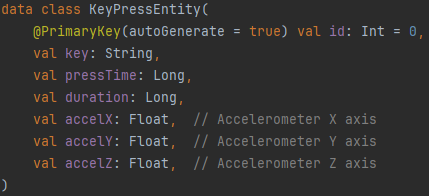
\includegraphics[width=0.8\linewidth]{images/DataModel.png}
		\caption{KeyPressEntity.kt}
		\label{fig:data_model_view}
	\end{figure}
	
	The \texttt{KeyPressEntity} is stored in a local SQLite database via Room.
	
	\item \textbf{View:} The user interface is implemented using \textbf{Jetpack Compose}, a declarative UI framework. Key components of the view contain:
	\begin{itemize}
		\item \textbf{Input Fields:} Lets users enter their credentials (University ID) and use the application for training or testing by pressing keys. 
		\item \textbf{Completion progress:} Informs users on what phase they are and displays progress of completion, linked to the \texttt{phasesCompleted} state in the \texttt{MainViewModel}.
		\item \textbf{Buttons:} Used for logging in, logging out, jumping phases and sending or downloading the data collected through training or testing stage.
	\end{itemize}
	\item \textbf{ViewModel:} This role is fulfilled by \texttt{MainViewModel}, which manages the application logic, handles interactions between the model and the view, and maintains the state of the app. \newline
	The \texttt{MainViewModel} class manages this operations through:
	\begin{itemize}
		\item \textbf{Logic Handling:} Methods such as \texttt{login()}, \texttt{logout()}, \texttt{clearDatabase()}, and \texttt{onKeyPress()} are responsible for managing user state and data.
		\item \textbf{State Management:} Stores states \texttt{isLoggedIn}, \texttt{username}, and \texttt{phasesCompleted}, which are used to dynamically update the user interface.
		\item \textbf{Data Management:} Connects with the \texttt{keyPressDao} database to process data. \texttt{onKeyPress} saves key press events into the database, \texttt{exportDataToTsv} exports the collected data into TSV files.
	\end{itemize}
\end{itemize}
In the app \textbf{DataStore} is used for storing login state and the user's ID. It has been implemented in \texttt{UserPreferences} class, and stores data such as:
\begin{itemize}
	\item \texttt{LOGGED\_IN\_KEY} - login state
	\item \texttt{USERNAME\_KEY} - user's ID.
\end{itemize}
\begin{figure}[H]
	\centering
	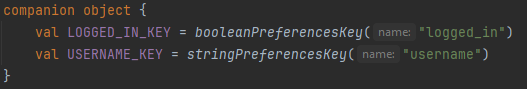
\includegraphics[width=0.8\linewidth]{images/CompanionObject.png}
	\caption{UserPreferences.kt}
	\label{fig:companion_object_view}
\end{figure}
This data is stored in the app's preferences file and can be accessed via dataStore object using:

\begin{itemize}
	\item \texttt{isLoggedIn} - returns login state as \texttt{Flow<Boolean>}
	\item \texttt{username} - returns user's ID as \texttt{Flow<String>}
	\item \texttt{setLoggedIn()} - saves login state and user's ID into DataStore
\end{itemize}

\begin{figure}[H]
	\centering
	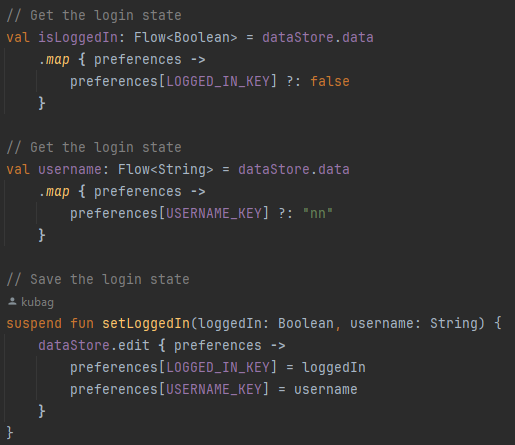
\includegraphics[width=0.8\linewidth]{images/UPFunctions.png}
	\caption{UserPreferences.kt}
	\label{fig:user_preferences_functions_view}
\end{figure}

The use of DataStore enabled the data to be stored securely, accessed and modified easily, and it is always available, which makes it a reliable and efficient way to manage user preferences and app state.

\subsection{User Interface Design}
The application design follows a minimalistic approach to make it intuitive and easy to use for everyone. 
\begin{itemize}
	\item 
	\texttt{Login Screen} \ref{fig:login_screen} \newline
	After launching the application for the first time, the user is presented with the \texttt{Login screen}. It contains \texttt{TextInput} field for entering the university ID, which was evenly distributed among contributors to simplify testing, and the \texttt{Log in} button which stores the ID and navigates the user to the \texttt{Home Screen}.
	\item 
	\texttt{Home Screen} \ref{fig:home_screen} \newline
	The home screen displays three buttons and a simple note explaining what the user should do. The \texttt{Logout} button navigates back to the \texttt{Login Screen}, while two other buttons lead to either testing or training screens.
	\item 
	\texttt{Training Screen} \ref{fig:training_screen} \newline
	The training screen is designed for collecting data for training purposes. It includes \texttt{TextInput} field for typing user input, a \texttt{Button} to proceed to the next phase, and \texttt{Text} indicators showing how many chars are needed to complete the phase (300 each phase) and how many phases remain (5 phases in total) to complete the process of collecting training data. Additionally, there are two notes instructing the user to maintain the writing style throughout the whole process and to change the position after each phase while writing (explained in subsection~\ref{sec:data_collection}). \newline
	To ensure that typing is done in the most natural way, the default android keyboard is used. 
	\item 
	\texttt{Testing Screen} \ref{fig:testing_screen} \newline
	The testing screen includes \texttt{TextInput} field for typing the test input, a \texttt{Button} that sends the input to the server and stores it locally, and \texttt{Text} indicators showing how many characters need to be written (in this case, 100). After fulfilling the requirements, the user sends their input to the server, which evaluates it against the trained model. The server then returns feedback and the user is presented with a recognition rate percentage on a circular progress bar and a message indicating whether the model recognised them or not \ref{fig:testing_screen_example}. 
\end{itemize}


\begin{figure}[H]
	\centering
	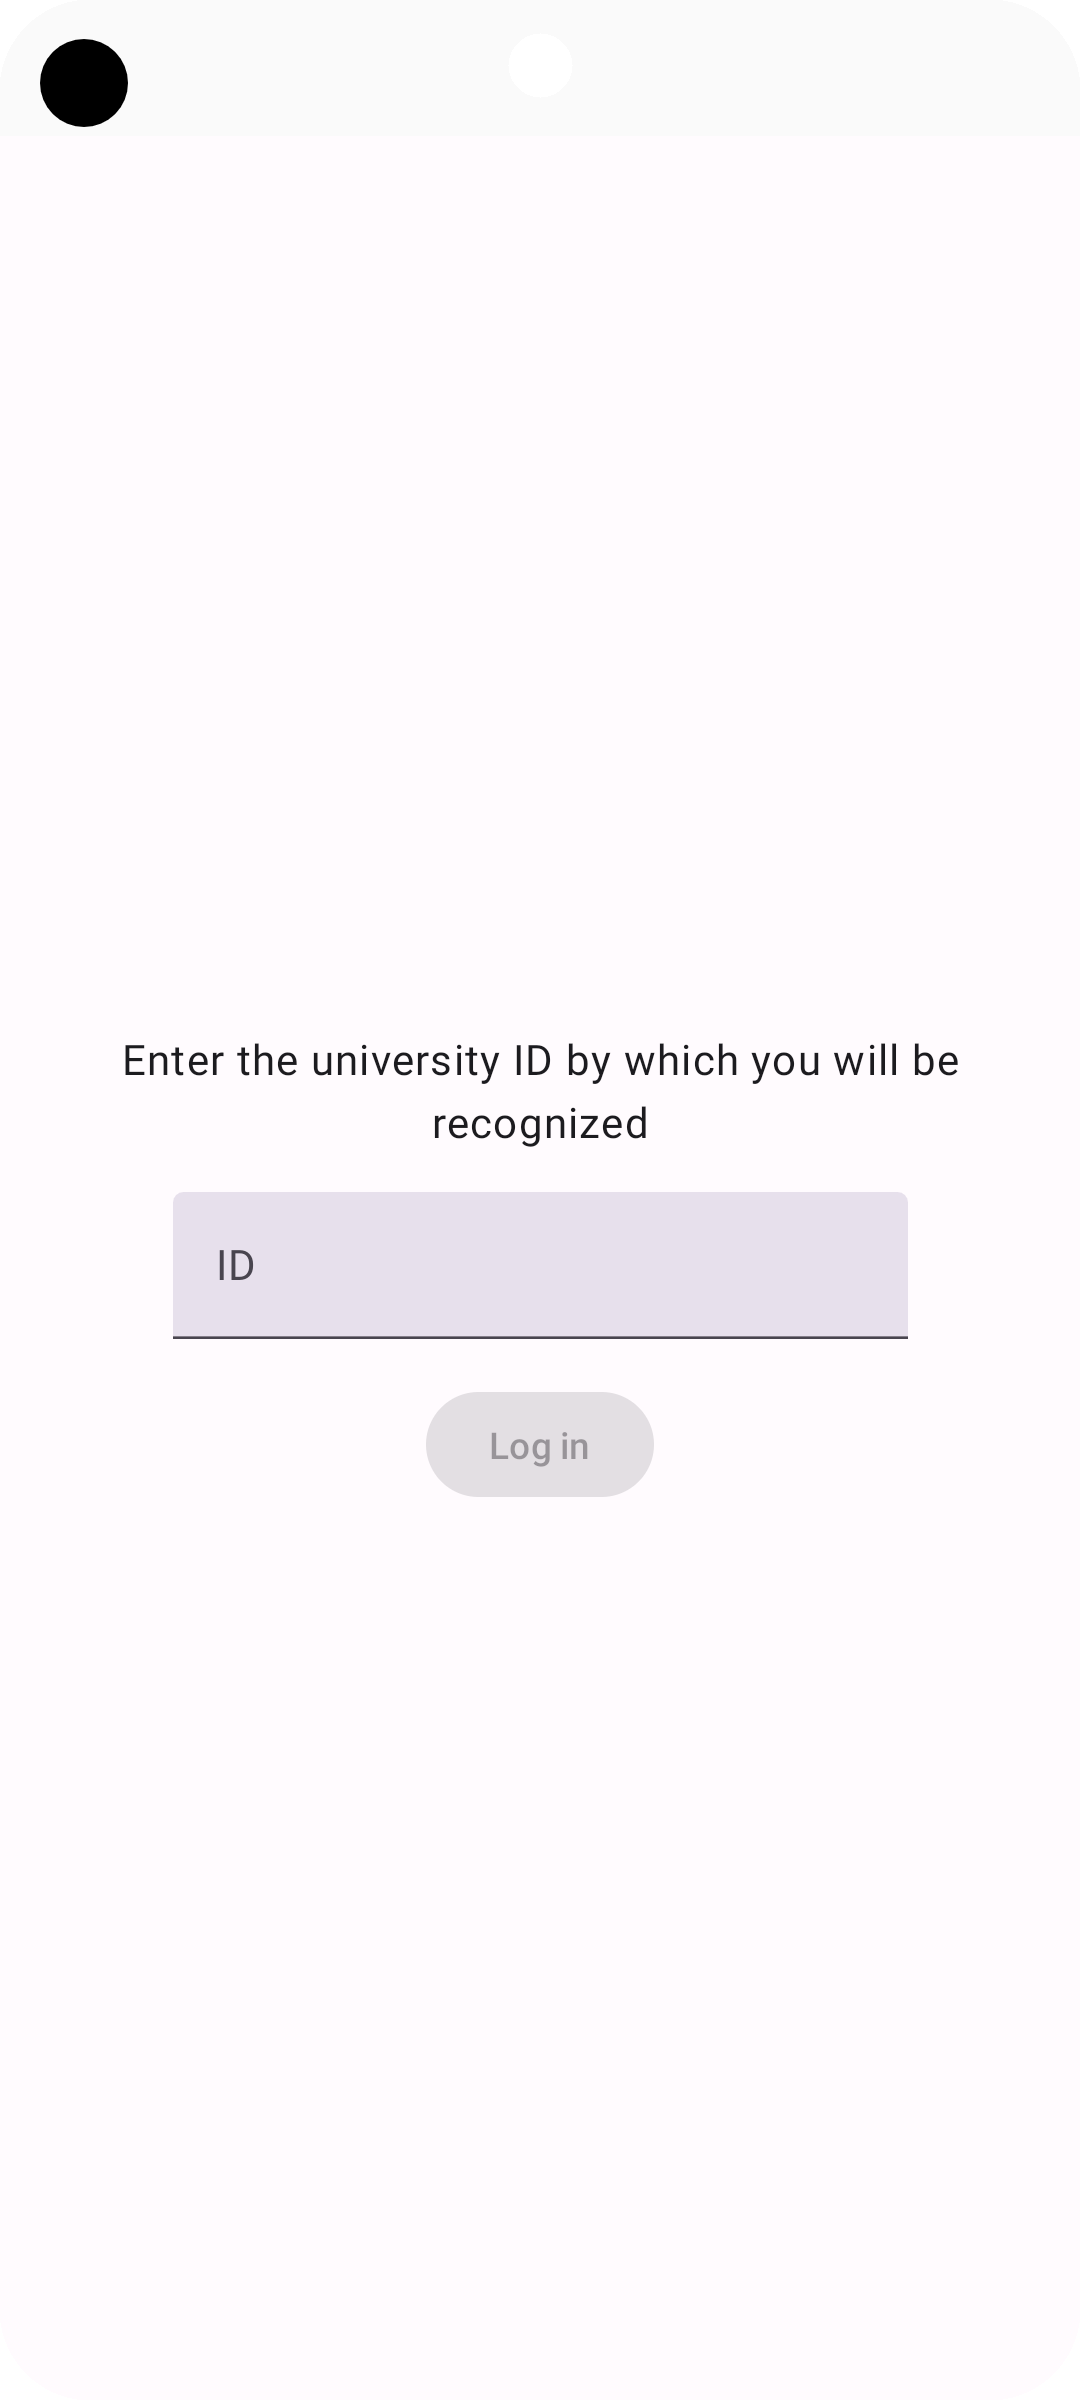
\includegraphics[width=0.32\linewidth]{images/login_screen.png}
	\caption{Login screen}
	\label{fig:login_screen}
\end{figure}

\begin{figure}[H]
	\centering
	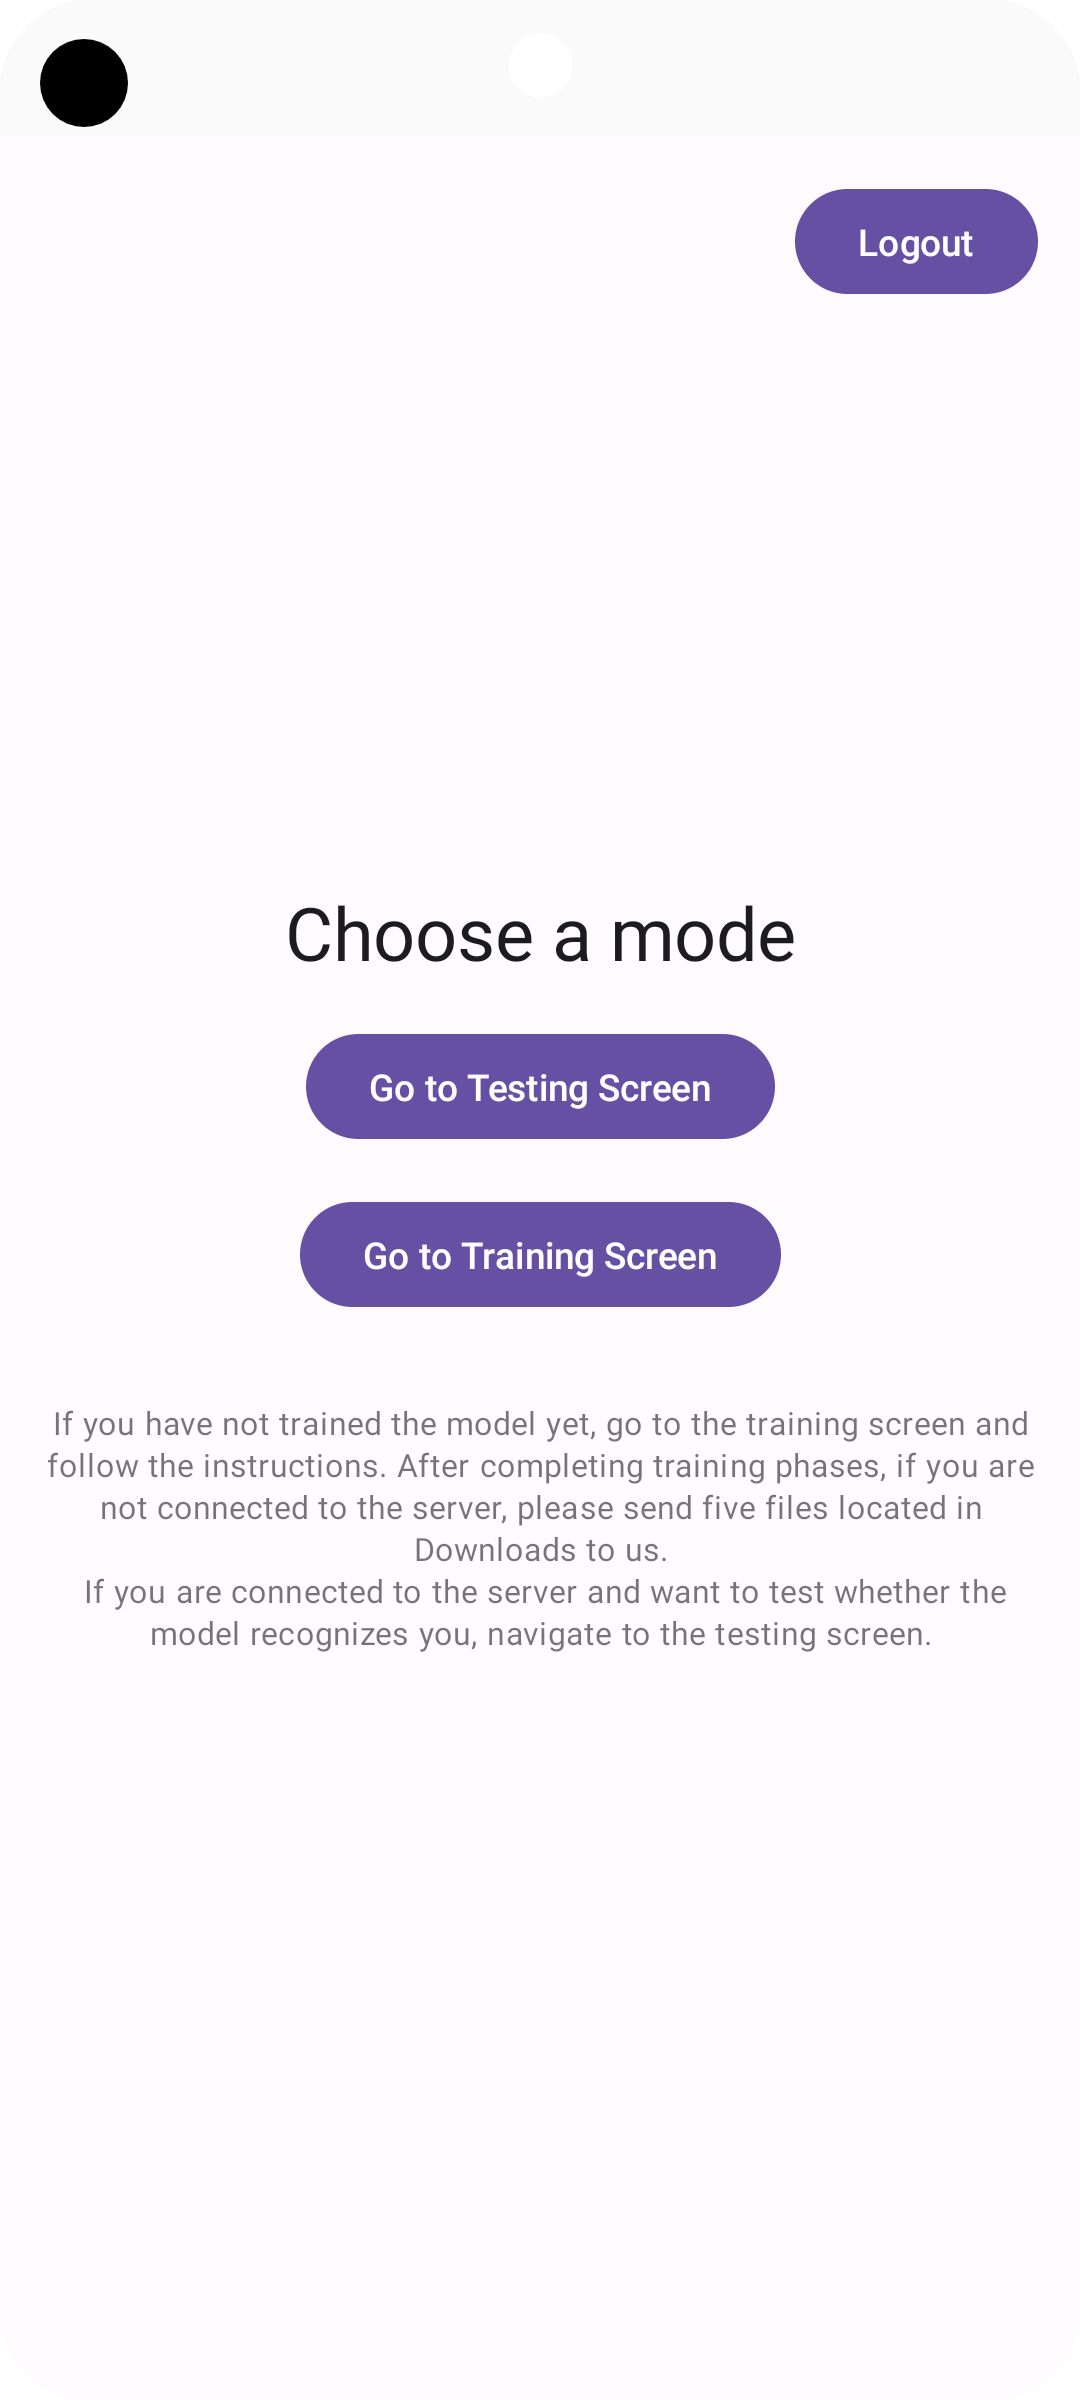
\includegraphics[width=0.32\linewidth]{images/home_screen.png}
	\caption{Home screen}
	\label{fig:home_screen}
\end{figure}

\begin{figure}[H]
	\centering
	
\includegraphics[width=0.32\linewidth]{images/training_screen.png}
	\caption{Training screen}
	\label{fig:training_screen}
\end{figure}

\begin{figure}[H]
	\centering
	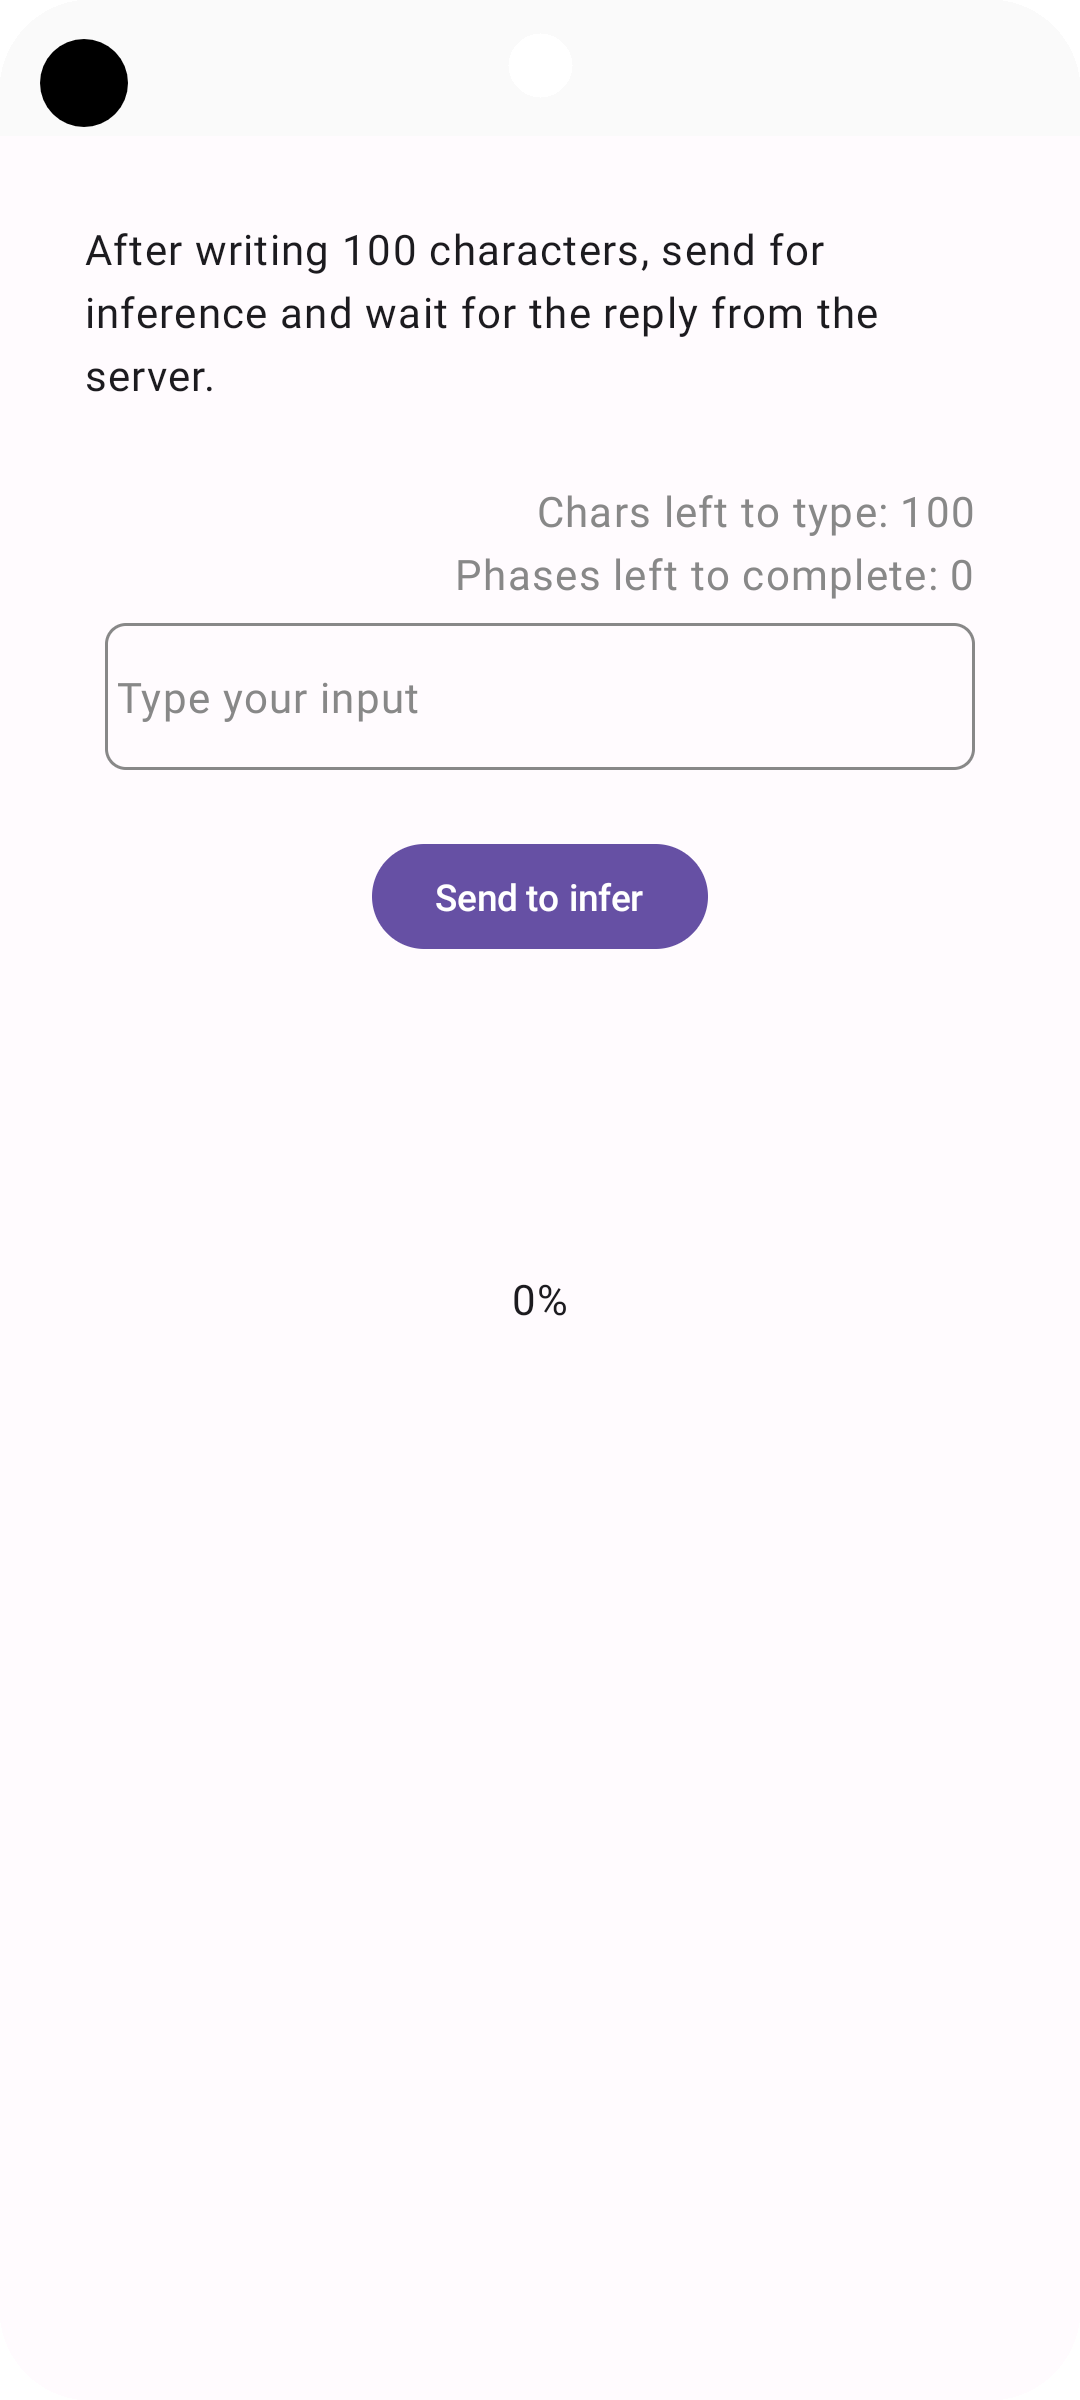
\includegraphics[width=0.32\linewidth]{images/testing_screen.png}
	\caption{Testing screen}
	\label{fig:testing_screen}
\end{figure}

\begin{figure}[H]
	\centering
	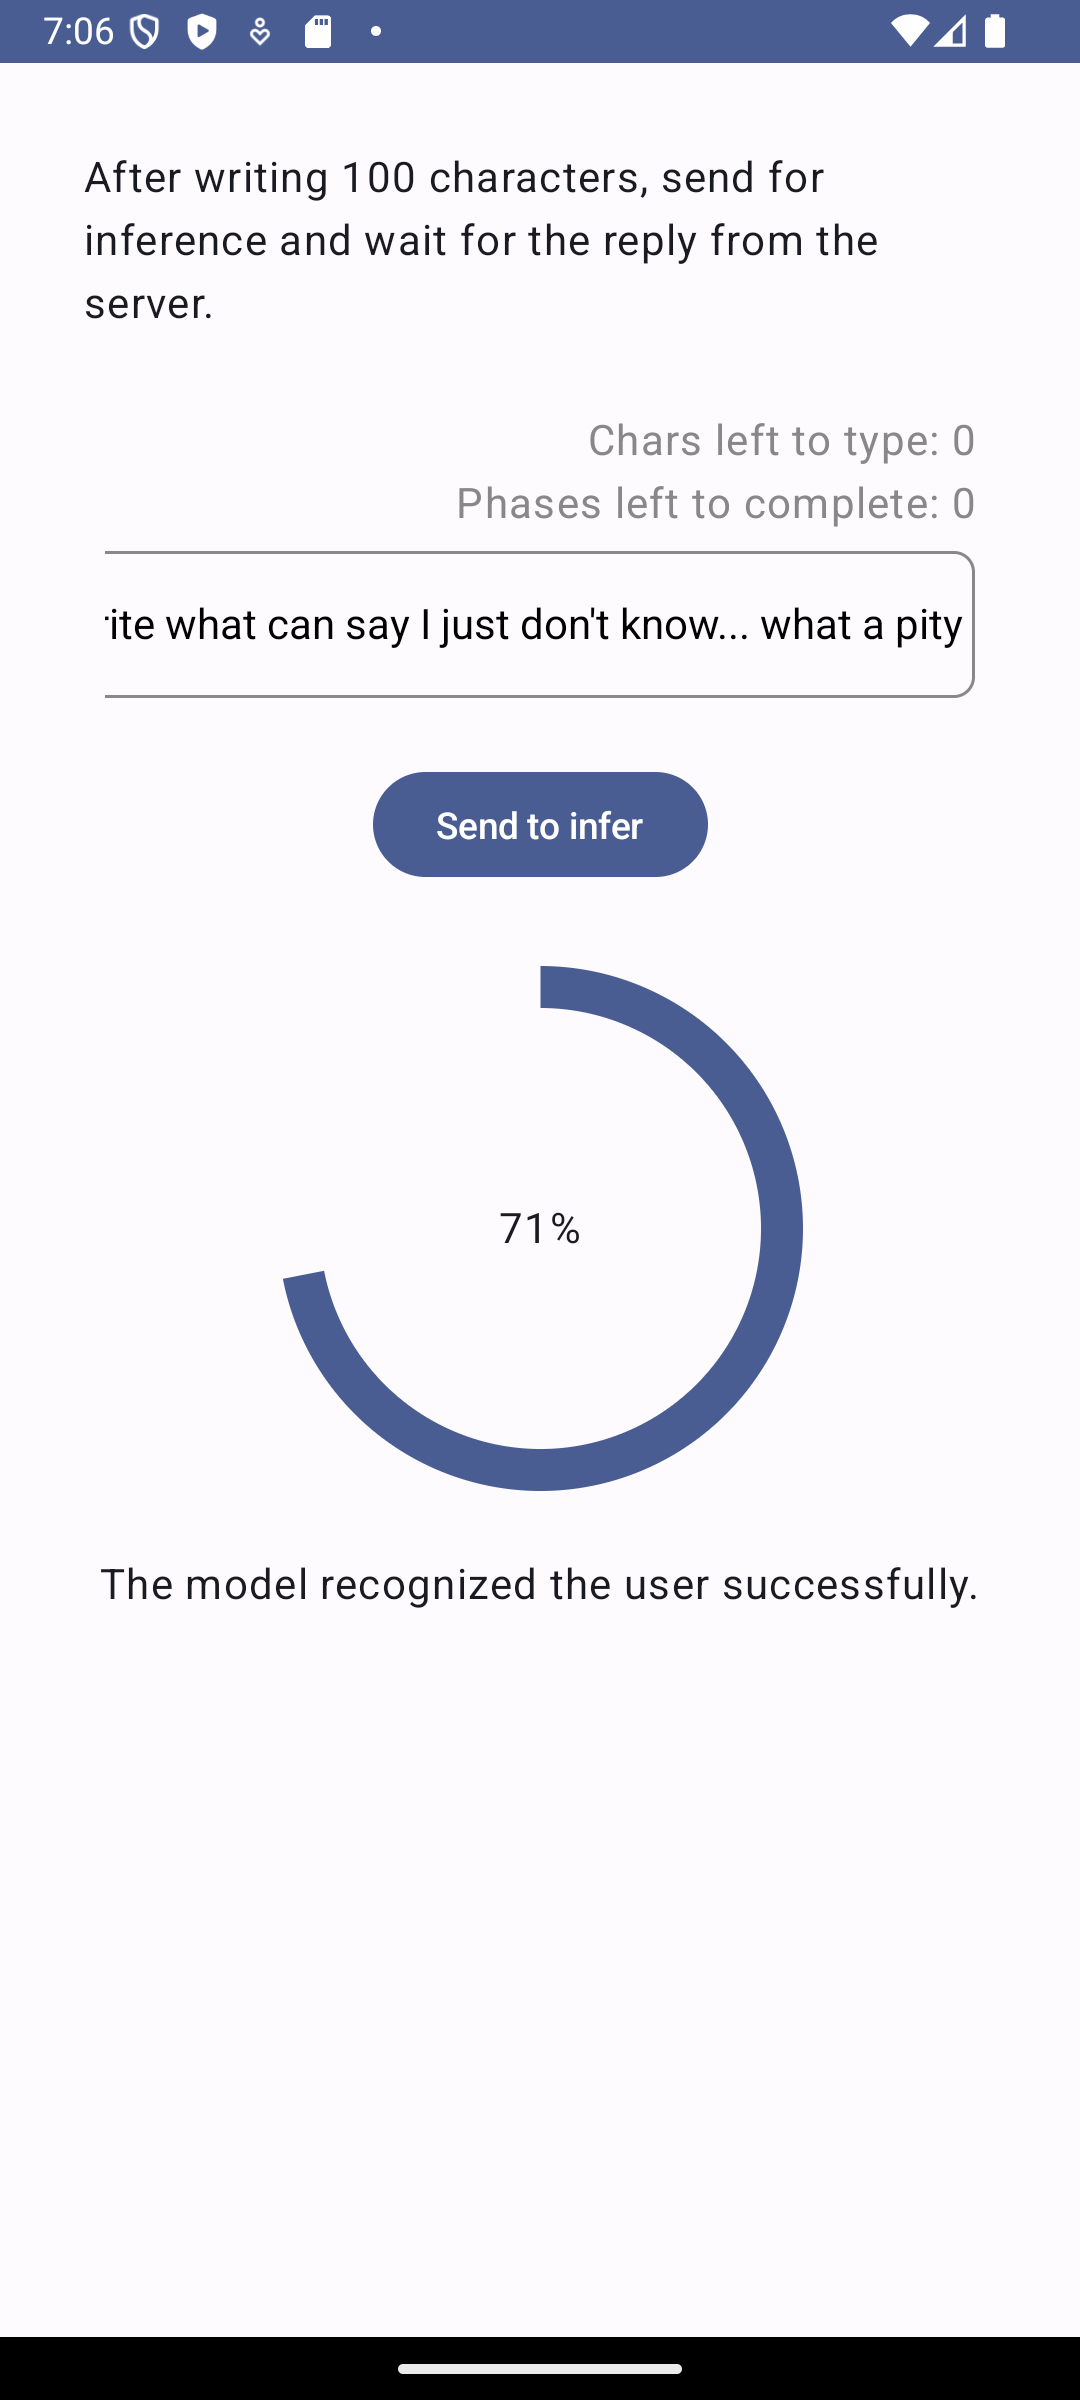
\includegraphics[width=0.32\linewidth]{images/testing_screen_example.png}
	\caption{Testing screen example}
	\label{fig:testing_screen_example}
\end{figure}

\subsection{Data Collection Process}
\label{sec:data_collection}
Data collection occurs in two stages, training and testing
\begin{itemize}
	\item 
	Training data collection begins on the \texttt{Training Screen} \ref{fig:training_screen}, where the user is asked to input meaningful sentences. The process consists of 5 phases. Each phase requires the user to type 300 characters. Once the requirement is met, the user progresses to the next phase until all 5 phases are completed (1500 characters in total). Additionally, there is a note instructing the user to maintain a consistent writing style throughout all phases. Also the user is asked to change their position after each phase while writing. This is important for accelerometer data collection (which is not used at the moment), as it helps exclude situations where the phone is lying on the table or being held in an atypical way.  
	\item 
	Testing data collection takes place on the \texttt{Testing Screen} \ref{fig:testing_screen}, where the user is required to write 100 characters, again in meaningful sentences. Once this is done, the testing phase is complete.
\end{itemize}
After each phase, the collected data is saved in a \texttt{.tsv} file, sent to the server, and stored locally in the phone's downloads directory. The \texttt{exportDataToTsv} \ref{fig:export_data_code} function from \texttt{MainViewModel.kt} handles the export of key press data. \newline Firstly it retrieves latest key press events using the \texttt{keyPressDao.getNLatestKeyPresses} method, converting the data into a \texttt{.tsv} format using the \texttt{keyPressesToTsv} function. \newline
Depending on which phase the user is in, the function determines the different type of operation to perform.
\begin{itemize}
	\item 
	If the user is in inference phase, the data will be used for inference.
	\item 
	If the user is in training phase, the data will be used for training.
	\item 
	If the number of completed phases exceeds the required amount, the function exits without performing any other action.
\end{itemize}

After processing data \texttt{saveTsvToDownloads} stores data locally, and \texttt{sendTsvToFastApi} sends data to the server (An example of the \texttt{.tsv} file containing the saved data is shown in Figure \ref{fig:tsv_example}). The username, and the relevant phase is included in the file name. \newline
This function ensures that after each phase of training and testing, the data is collected, stored, and transmitted.

\begin{figure}[H]
	\centering
	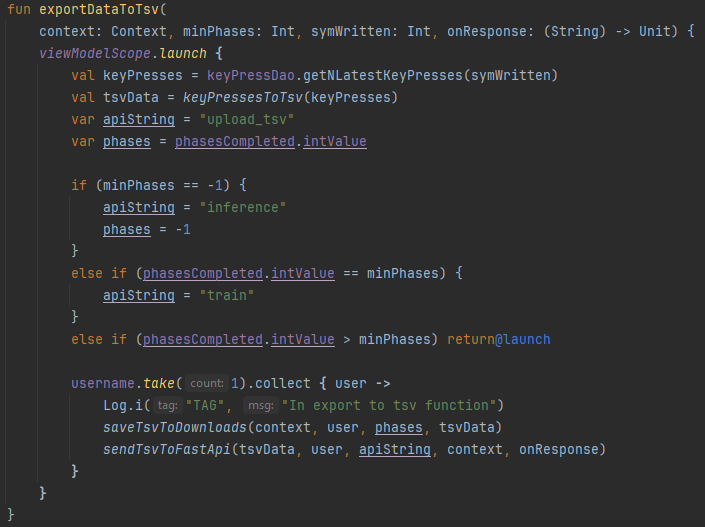
\includegraphics[width=0.8\linewidth]{images/ExportData.png}
	\caption{MainViewModel.kt}
	\label{fig:export_data_code}
\end{figure}

\begin{figure}[H]
	\centering
	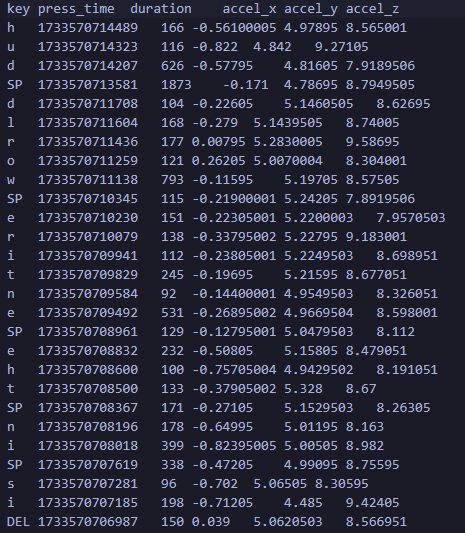
\includegraphics[width=0.8\linewidth]{images/data_example.png}
	\caption{An example of the \texttt{.tsv} file containing saved data.}
	\label{fig:tsv_example}
\end{figure}

\subsection{Communication with the server}

The application communicates with the server using an HTTPS connection.
\begin{itemize}
	\item 
	\textbf{Server URL and Request Structure}
	\begin{itemize}
		\item 
		The server is accessed via an HTTPS endpoint. The base URL is defined as \newline \texttt{https://192.168.1.100:8000}.
		\item 
		The API endpoint is dynamically created with the use of a route and query parameters to the base URL. For example, the endpoint for sending data contains the username as a query parameter: \newline
		\texttt{https://192.168.1.100:8000/<api\_string>?username=<username>}
		\item 
		The data is sent using the POST method.
	\end{itemize}
	\item
	\textbf{Data format} \newline
	The data sent to the server is stored in \texttt{.tsv} (tab-separated values) file, containing headers and the detailed information about key presses.
	\item 
	\textbf{Secure Connection Setup}
	\begin{itemize}
		\item 
		The application uses \texttt{OkHttpClient} library for handling network requests.
		\item 
		A \texttt{.cert} certificate (stored in \texttt{res/raw/cert}) is used to establish a secure and trustworthy \texttt{SSL/TLS} connection.
	\end{itemize}
	\item 
	\textbf{Sending request}
	\begin{itemize}
		\item 
		Requests are executed asynchronously using the \texttt{enqueue} method.
		\item 
		If successful, the server's response is processed, and the application displays the result to the user.
		\item 
		On failure, the error is logged, and the user is notified.  
	\end{itemize}
	\item 
	\textbf{Error Handling}
	\begin{itemize}
		\item 
		Network errors (e.g., problems with connection) and server errors are logged for easier debugging.
		\item 
		A callback system is implemented to communicate feedback to the user. 
	\end{itemize}
	
	
\end{itemize}


\chapter{GCN Model}

In modern Machine Learning, a popular type of Neural Network is a Convolutional Neural Network. Such networks generally operate on grids. A Convolutional Neural Network (CNN) has a fixed node ordering -- some input must firstly be mapped into a grid to be used with a CNN. There are ways to map many types of data into such format. Examples of researchers using CNNs for keystroke dynamics data include Sharma et al. \cite{Shar2023} or Lu et al. \cite{Lu2020}. In Lu et al. this involved applying the convolution layers over feature vectors, which were constructed in the following manner: for pairs of keys pressed in succesion in the sequence, a feature vector is created with fields: ID of first key, ID of second key, hold duration of first key, hold duration of second key, DD time (time between first press and second press) and DU time (time between first press and second release). After applying the CNN layer, GRU layers were used.

In this project, the goal was to use the graph networks that can naturally arise from keystroke data to -- on a graph level -- try to infere the users identity. The main difference was that the use of any keyboard already installed on the user's mobile phone causes some problems with gathering keystroke temporal data, as mentioned in the second chapter. Because of that, this project used mappings involving only key ...

Moreover, this project focused on creating an ensable of models, one model for each user that performs binary classification rather than one large model for multiclass classification. This decision was made for several reasons. Firstly, such scheme allows for models to be trained on demand, as soon as a new user provides all the training data to the mobile aplication. Secondly, new users do not force the whole model to be retrained, as only one new model needs to be created, and provided all models have learned their target users sufficiently, they would be able to reject such new users. Lastly, the one user per model scheme allows for inference to take place locally, on the target user's device. This would remove the need for remote communication with the server, thus increasing the mobile aplication's reliablity and security. On device inference is an area of active research, such as \myworries{TODO citation needed}, the complexity of such solution was deemed to great and outside the scope of this project.

\section{Choosing features for Neural Network model}
\myworries{TODO Some introdutions}


\subsection{Data exploration}
\myworries{All data analisys on the input goes here}

\subsection{Graph creation and feature encoding}
The input for graph creation consists of two main parts, the duration of time between individual key presses, and the character of the key that was pressed.
A natural way to represent such input was to map each unique character in the input sequence to a node in the graph. 
Directed edges were added between nodes that represent characters appearing after each other in the input sequence. 
\myworries{TODO: add example graph visualization here}
Each time the same pair of characters appears in the input text it maps to the same edge. For each such pair, the duration is added to a list attributes for that edge, which will be aggregated in later stages, to a form suitable for the GCN model. It would also be possible to model such pairs using a multiedge graph, as such models have been shown to perform well in other domains \myworries{TODO zacytuj "multi-edge graph for convolutional networks for power systems}. However we did not consider this approach. 

\myworries{TODO maybe visualization}
The structure of the resulting graph depends highly on the length of the input sequence. A shorter sequence produces smaller and sparser graphs, while a longer input sequences result in graphs with more nodes and edges. 

\myworries{Citation needed - some RNN paper that sequences of keys are important}\\

\subsubsection{edge atributes encoding}
In order for the graph to be a valid input for a GCN network, edge attributes need to be converted into node features. We found two ways to encode aggregate this information into node features.\\  
For each node $i$:
\begin{enumerate}
	\item Two values representing the average duration before and after the key represented by $i$ was pressed.
	\item Add two-dimensional vector of values, of size [number of allowed characters, 2]. Each key that can be found in the input is assigned a number. The $n$'th row in the vector corresponds to a node, with a key assigned the number $n$, now called node $j$. The $n$'th row contains two values: the average duration on the edge from $i$ to $j$ and the average duration on the edge from $j$ to $i$. The values for which edges do not exist were assigned 0.
\end{enumerate}
The clear difference between these two approaches is the level of aggregation. Method $1$ aggregates all the edge information into 2 values, while method $2$ aggregates it into a vector of values, although it imposes some limitations, such as assigning each key a unique index into this input vector. Furthermore method $2$ increases the overall size of the input data and complexity of the model.


\subsubsection{Character atributes encoding}
As this project focuses on recognizing users of the Polish language, the character encodings were designed to make use of this fact. For the purpose of encoding, characters were divided into several groups:\\
\begin{itemize}
	\item Letters -- characters \textit{a-z}, including diacritics.
	\item Numbers -- characters \textit{0-9}
	\item Special characters -- \textit{space}, \textit{tab}, \textit{newline}, \textit{backspace}, \textit{dot}, \textit{comma}, \textit{exclamation mark}, \textit{question mark}.
	\item Symbols -- \textit{*}, \textit{\#}, \textit{@}, \textit{:}, \textit{;},   \textit{'}, \textit{"}, \textit{(}, \textit{)}, \textit{[}, \textit{]}, \textit{\{}, \textit{\}}, \textless, \textgreater, \textit{/}, \textit{$\backslash$}, \textit{|}, \&, \%, \textit{\$}, \textit{\^}, \~, \textit{\_}, \textit{+}, \textit{-}, \textit{=}. 
	\item Others -- all other symbols.
\end{itemize}
Similarly, there is more than one way to encode key information into node features.
We considered three methods, all being variations on a one-hot encoding of keys:
\begin{enumerate}
	\item Classic one-hot representation. Each unique cased character is mapped to different column in the vector, except for characters in the \textit{Others} group, which map to one extra column.
	\item Small alphabet representation. One hot encoding for cased \textit{Letters} and \textit{Special characters}. \textit{Numbers} map to one column in the vector, \textit{Symbols} and \textit{Others} map to one column in the vector.
	\item Base letter representation. All \textit{Letters} are converted lower case, diacritical marks are removed. These transformed letters are encoded in a one-hot vector. \textit{Numbers} map to one column in the vector, \textit{Symbols} and \textit{Others} map to one column in the vector. Two additional columns are added to the input, one indicates whether the original character was a capitalized letters, the second whether it had a diacritical marks.
\end{enumerate}

\myworries{Citation needed: That paper that said node id's are nice}.
Again as before, these methods differ by degree of aggregation. Methods $2$ and $3$ group certain letters together, mapping multiple characters to the same values, while method $1$ provides a unique, one hot encoded identifier for each node. \myworries{Cication} found that such node identifiers helped the model to learn certain structures in the data. However, \myworries{Slajdy z stanfordu ze tylko jak jest ograniczona liczba liter} notes, that providing node identifiers as input features work well only for a small and known set of possible input nodes. While this requirement appears to hold true for this specific task, we found this is not the case. Many letters, which appear to be common, in fact do not appear in our dataset. \myworries{TODO Which chars never appear}. This means that the behavior of the models would be unpredictable for nodes with such identifiers.
Some characters, for example \myworries{EXMAPLEEEE like '('}, appear only once, leading models to overfit and generalize poorly.
Method $3$ was specifically designed to deal with the low number of appearances of certain characters, especially uppercase letters. However, the extra column still allows for distinguishing between lower and uppercase variants of the same letter, which is important as the time to input these symbol differs greatly. \myworries{Avg time for uppercase and lowercase letters}
Moreover, method $3$ directly exposes the use of diacritical marks, which, similarly to uppercase letter, take longer to input \myworries{Gimme DATAAAAA}. 
\myworries{Ładne zdanie które mówi wooow, diarectical marks are nice in polish, maybe data}

\myworries{ADD histogram of how many times each character appears}\\
\myworries{ADD Which chars never appear}


\subsection{Feature selection - accelerometer data}
To improve the possible performance of the model, and to make further use of the capabilities of the mobile platform, we considered using accelerometer data as a input feature for the model.
This portion of the input data comprised of three values, a measurement of the acceleration in the x, y and z plane at the moment a keystroke was registered. 
These values were aggregated as an average for each node. Although these models performed well during training, quickly reaching low loss values, they failed to generalize, performing worse on 
validation and test datasets. 

\myworries{TODO, some accelerometer data here}
For this reason, accelerometer data was not used for training and evaluating models discussed later.




\section{Graph Convolutional Network for user recognition}

In modern Machine Learning, a popular type of Neural Network is a Convolutional Neural Network. Such networks generally operate on grids. A Convolutional Neural Network (CNN) has a fixed node ordering -- some input must firstly be mapped into a grid to be used with a CNN. There are ways to map many types of data into such format. Examples of researchers using CNNs for keystroke dynamics data include Sharma et al. \cite{Shar2023} or Lu et al. \cite{Lu2020}. In Lu et al. this involved applying the convolution layers over feature vectors, which were constructed in the following manner: for pairs of keys pressed in succesion in the sequence, a feature vector is created with fields: ID of first key, ID of second key, hold duration of first key, hold duration of second key, DD time (time between first press and second press) and DU time (time between first press and second release). After applying the CNN layer, GRU layers were used.

In this project, the goal was to use the graph networks that can naturally arise from keystroke data to -- on a graph level -- try to infere the users identity. The main difference was that the use of any keyboard already installed on the user's mobile phone causes some problems with gathering keystroke temporal data, as mentioned in the second chapter. Because of that, this project used mappings involving only key ...

TODO for IW: anything and everything about the model, the inner structure, the feature extraction can also go there, ask FK how you want to split these subjects up. FK will probably also check in with something here.

\myworries{TODO: moreso about network structure, less about feature extraction}


\section{Model selection}



\section{Model fine-tuning and hyperparameters - metrics}

TODO for IW: write about the fine-tuning process, the metrics used and why are they used, cross-validations used etc. You can also post some hyperparam statistics here.

\subsection{Metrics used}

\section{Testing model on users}

TODO for xxx: when the tests are done (hopefully a week) we will discuss this. Also, there could be a part about many-users recognition.

\subsection{Cross-smartphone user validation}
TODO: what happens if two users train on smartphones that are not their own? What happens, if they cross-use their original model on another phone?

\subsection{Discussion}
TODO: discuss the findings.

\chapter{Conlusion}

TODO for JG: not needed now, will write after the user tests are done.


%--------------------------------------
% Literatura
%--------------------------------------

\bibliographystyle{plain}{\raggedright\sloppy\small\bibliography{bibliography}}

%--------------------------------------
% Dodatki
%--------------------------------------

\cleardoublepage\appendix%

%--------------------------------------
% Informacja o prawach autorskich
%--------------------------------------

\end{document}
